% =============================================================================
% DAGs causales del ARTICULO longitudinal, en TikZ.
%
% La fuente de verdad conceptual es docs/dags-longitudinales.md, escrito en
% Mermaid: se versiona en texto, se lee en GitHub sin compilar nada y no se
% desincroniza. Este archivo es su traduccion tipografica para la figura del
% manuscrito, que va en INGLES a diferencia de los de la tesis.
%
% Convencion de Hernan y Robins: el RECUADRO indica que el analisis condiciona
% sobre esa variable.
%
% Compilar:  lualatex dags_longitudinales.tex
% =============================================================================
\documentclass[border=10pt]{standalone}

\usepackage{amsmath}   % \text{} en subindices
\usepackage{fontspec}
\setmainfont{Latin Modern Roman}
\setsansfont{Latin Modern Sans}
\usepackage{tikz}
\usetikzlibrary{arrows.meta,positioning,calc,fit,backgrounds}

% Paleta identica a la de las demas figuras del proyecto.
\definecolor{marino}{HTML}{003366}
\definecolor{marinocla}{HTML}{E8EDF3}
\definecolor{grisosc}{HTML}{404040}
\definecolor{gris}{HTML}{7A7A7A}
\definecolor{griscla}{HTML}{D0D0D0}
\definecolor{alerta}{HTML}{8C3A2E}
\definecolor{alertacla}{HTML}{F7ECEA}
\definecolor{verde}{HTML}{2F6B4F}
\definecolor{verdecla}{HTML}{E7F1EC}

\tikzset{
  every node/.style      = {font=\sffamily\small},
  nodo/.style            = {draw=grisosc, fill=white, rounded corners=2pt,
                            minimum height=8mm, minimum width=15mm,
                            inner sep=3pt, align=center, line width=0.5pt},
  rasgo/.style           = {nodo, draw=marino, fill=marinocla, line width=0.9pt},
  hallado/.style         = {nodo, draw=verde, fill=verdecla, line width=0.9pt},
  nomedida/.style        = {nodo, draw=gris, dashed, fill=white},
  censura/.style         = {nodo, draw=alerta, fill=alertacla, line width=0.9pt},
  % El doble recuadro es la notacion de Hernan y Robins para el condicionamiento.
  condicionado/.style    = {nodo, double, double distance=1.2pt, draw=marino},
  flecha/.style          = {-{Stealth[length=2.2mm]}, draw=grisosc, line width=0.6pt},
  espuria/.style         = {-{Stealth[length=2.2mm]}, draw=gris, dashed,
                            line width=0.6pt},
  nula/.style            = {-{Stealth[length=2.2mm]}, draw=griscla, dotted,
                            line width=0.6pt},
  doble/.style           = {{Stealth[length=2.2mm]}-{Stealth[length=2.2mm]},
                            draw=marino, line width=0.8pt},
  rot/.style             = {font=\sffamily\scriptsize, text=grisosc,
                            inner sep=1.5pt, fill=white},
  titulo/.style          = {font=\sffamily\bfseries\small, text=black, anchor=west},
  pie/.style             = {font=\sffamily\scriptsize, text=grisosc,
                            anchor=west, align=left},
}

\begin{document}
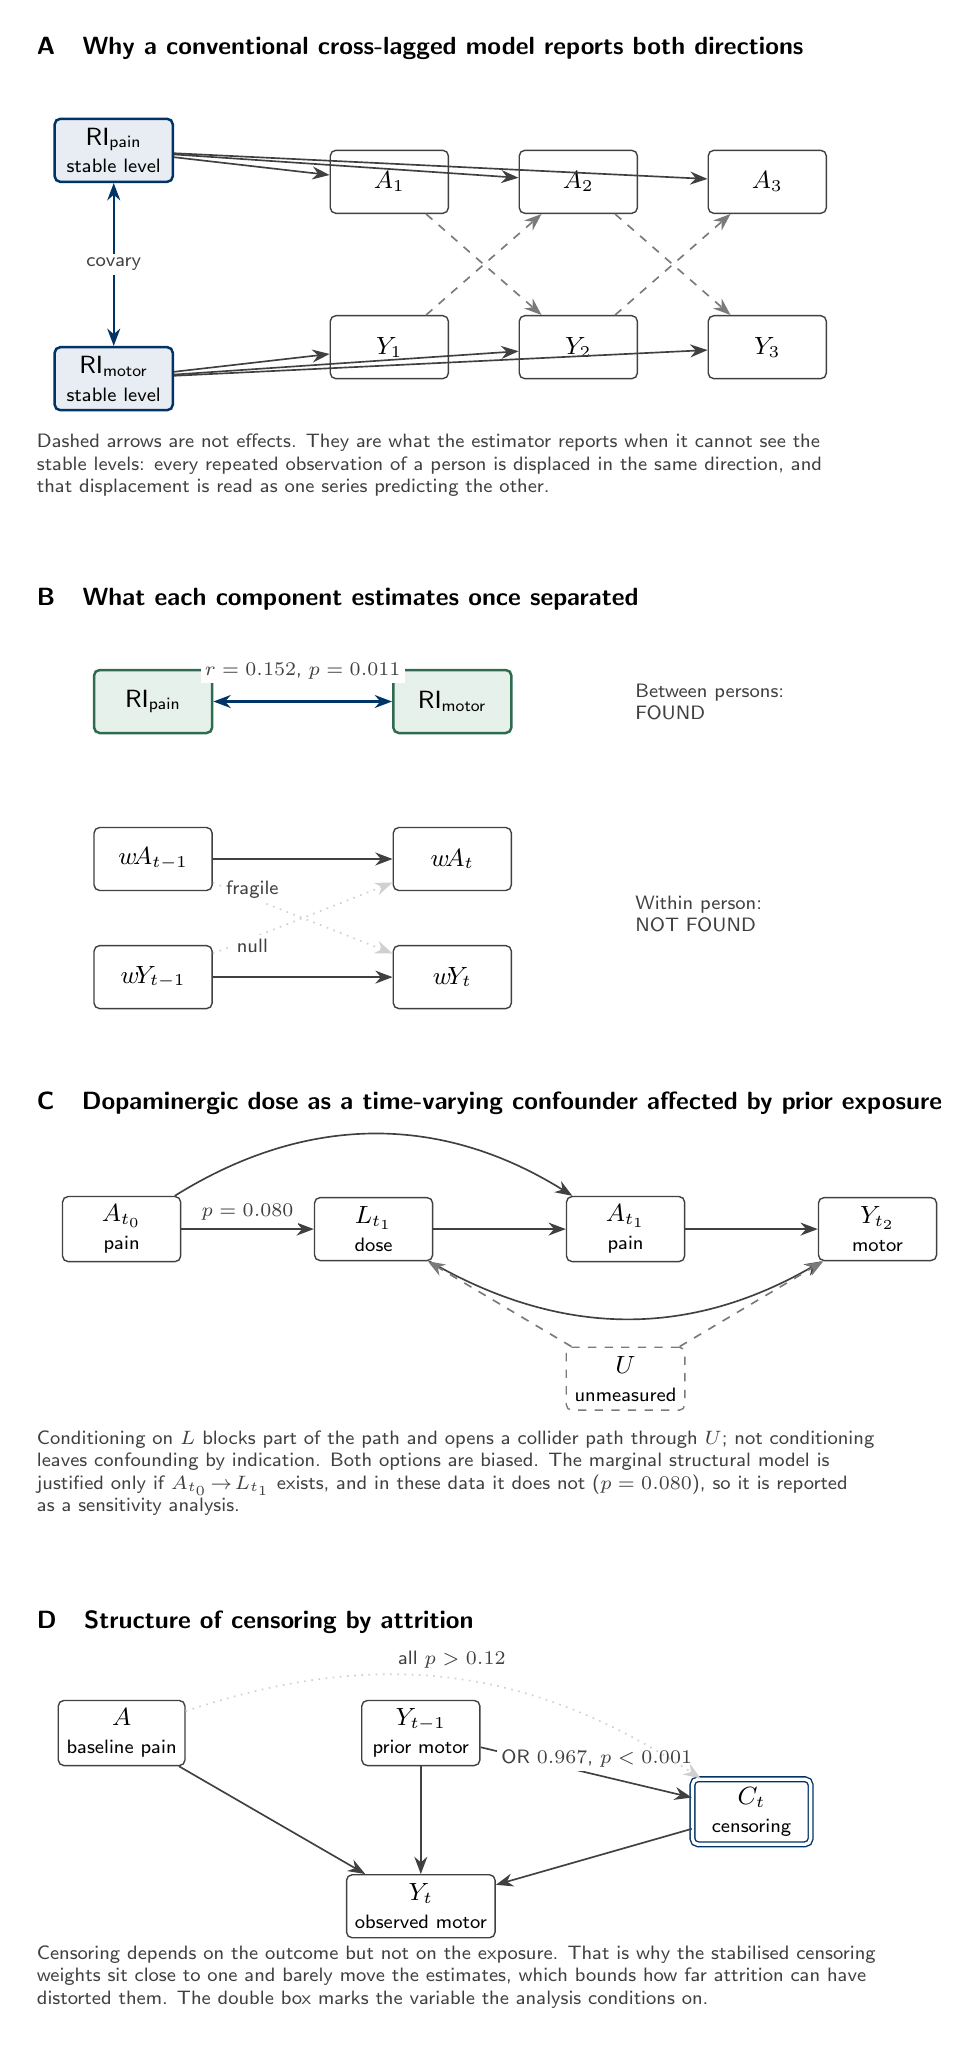
\begin{tikzpicture}[node distance=9mm]

% =============================================================================
% PANEL A. Por que el panel cruzado clasico fabrica bidireccionalidad
% =============================================================================
\node[titulo] (tA) at (0,0) {A\quad Why a conventional cross-lagged model reports both directions};

\node[rasgo] (ria) at (1.1,-1.3) {RI$_{\text{pain}}$\\[-1pt]{\scriptsize stable level}};
\node[rasgo] (riy) at (1.1,-4.2) {RI$_{\text{motor}}$\\[-1pt]{\scriptsize stable level}};

\node[nodo] (a1) at (4.6,-1.7) {$A_1$};
\node[nodo] (a2) at (7.0,-1.7) {$A_2$};
\node[nodo] (a3) at (9.4,-1.7) {$A_3$};
\node[nodo] (y1) at (4.6,-3.8) {$Y_1$};
\node[nodo] (y2) at (7.0,-3.8) {$Y_2$};
\node[nodo] (y3) at (9.4,-3.8) {$Y_3$};

\foreach \t in {a1,a2,a3} \draw[flecha] (ria) -- (\t);
\foreach \t in {y1,y2,y3} \draw[flecha] (riy) -- (\t);
\draw[doble] (ria) -- node[rot,pos=0.5] {covary} (riy);

\draw[espuria] (a1) -- (y2);
\draw[espuria] (y1) -- (a2);
\draw[espuria] (a2) -- (y3);
\draw[espuria] (y2) -- (a3);

\node[pie] at (0,-5.3) {Dashed arrows are not effects. They are what the estimator reports when it cannot see the\\
stable levels: every repeated observation of a person is displaced in the same direction, and\\
that displacement is read as one series predicting the other.};

% =============================================================================
% PANEL B. Que estima cada componente una vez separados
% =============================================================================
\node[titulo] (tB) at (0,-7.0) {B\quad What each component estimates once separated};

\node[hallado] (bria) at (1.6,-8.3) {RI$_{\text{pain}}$};
\node[hallado] (briy) at (5.4,-8.3) {RI$_{\text{motor}}$};
\draw[doble] (bria) -- node[rot,pos=0.5,yshift=11pt] {$r=0.152$, $p=0.011$} (briy);
\node[pie] at (7.6,-8.3) {Between persons:\\FOUND};

\node[nodo] (wa1) at (1.6,-10.3) {$w\!A_{t-1}$};
\node[nodo] (wa2) at (5.4,-10.3) {$w\!A_{t}$};
\node[nodo] (wy1) at (1.6,-11.8) {$w\!Y_{t-1}$};
\node[nodo] (wy2) at (5.4,-11.8) {$w\!Y_{t}$};
\draw[flecha] (wa1) -- (wa2);
\draw[flecha] (wy1) -- (wy2);
\draw[nula] (wa1) -- node[rot,pos=0.22,yshift=3pt] {fragile} (wy2);
\draw[nula] (wy1) -- node[rot,pos=0.22,yshift=-3pt] {null} (wa2);
\node[pie] at (7.6,-11.0) {Within person:\\NOT FOUND};

% =============================================================================
% PANEL C. La dosis como confusor afectado por la exposicion previa
% =============================================================================
\node[titulo] (tC) at (0,-13.4) {C\quad Dopaminergic dose as a time-varying confounder affected by prior exposure};

\node[nodo] (ca0) at (1.2,-15.0) {$A_{t_0}$\\[-1pt]{\scriptsize pain}};
\node[nodo] (cl1) at (4.4,-15.0) {$L_{t_1}$\\[-1pt]{\scriptsize dose}};
\node[nodo] (ca1) at (7.6,-15.0) {$A_{t_1}$\\[-1pt]{\scriptsize pain}};
\node[nodo] (cy2) at (10.8,-15.0) {$Y_{t_2}$\\[-1pt]{\scriptsize motor}};
\node[nomedida] (cu) at (7.6,-16.9) {$U$\\[-1pt]{\scriptsize unmeasured}};

\draw[flecha] (ca0) -- node[rot,pos=0.5,yshift=6pt] {$p=0.080$} (cl1);
\draw[flecha] (cl1) -- (ca1);
\draw[flecha] (ca1) -- (cy2);
\draw[flecha] (ca0) to[bend left=32] (ca1);
\draw[flecha] (cl1) to[bend right=30] (cy2);
\draw[espuria] (cu) -- (cl1);
\draw[espuria] (cu) -- (cy2);

\node[pie] at (0,-18.1) {Conditioning on $L$ blocks part of the path and opens a collider path through $U$; not conditioning\\
leaves confounding by indication. Both options are biased. The marginal structural model is\\
justified only if $A_{t_0}\!\rightarrow\!L_{t_1}$ exists, and in these data it does not ($p=0.080$), so it is reported\\
as a sensitivity analysis.};

% =============================================================================
% PANEL D. La censura por atricion
% =============================================================================
\node[titulo] (tD) at (0,-20.0) {D\quad Structure of censoring by attrition};

\node[nodo] (da) at (1.2,-21.4) {$A$\\[-1pt]{\scriptsize baseline pain}};
\node[nodo] (dy0) at (5.0,-21.4) {$Y_{t-1}$\\[-1pt]{\scriptsize prior motor}};
\node[censura,condicionado] (dc) at (9.2,-22.4) {$C_t$\\[-1pt]{\scriptsize censoring}};
\node[nodo] (dy1) at (5.0,-23.6) {$Y_t$\\[-1pt]{\scriptsize observed motor}};

\draw[flecha] (dy0) -- node[rot,pos=0.55,yshift=6pt] {OR $0.967$, $p<0.001$} (dc);
\draw[nula] (da) to[bend left=26] node[rot,pos=0.5,yshift=7pt] {all $p>0.12$} (dc);
\draw[flecha] (dy0) -- (dy1);
\draw[flecha] (da) -- (dy1);
\draw[flecha] (dc) -- (dy1);

\node[pie] at (0,-24.5) {Censoring depends on the outcome but not on the exposure. That is why the stabilised censoring\\
weights sit close to one and barely move the estimates, which bounds how far attrition can have\\
distorted them. The double box marks the variable the analysis conditions on.};

\end{tikzpicture}
\end{document}
